\section{Person Isolation}
\label{person isolation}
This section details the creation of a method to isolate a person from the background data. An advantage of using a Kinect over another camera is that the Kinect is able to isolate a skeleton associated with a person. This skeleton meant that the group did not have to make use of computationally heavy computer vision algorithms to isolate a person \todo{example}.\\

Instead, the method developed used the skeleton to determine the approximate depth of the person (using the HipCenter joint). Any point whose depth value is outside a delta (specifically 400) of the HipCenter is discarded.

\begin{figure}[h]
\begin{center}
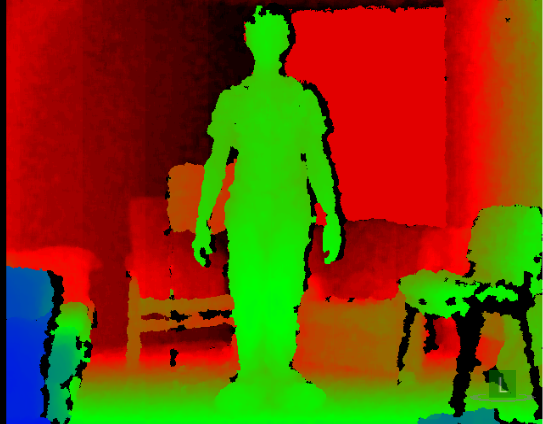
\includegraphics[scale=0.75]{./design/parse1}
\end{center}
\caption{The Basic Idea of UWAN-MAC.}
\label{fig:basicidea}
\end{figure} 

to determine the left and right most point of the person (i.e. the persons hands) and exclude everything that was outside this range.